\section{Design}\label{design}

%% This section is too basic, and therefore is boring because most readers
%% will already know it.  It also delays the interesting parts of the paper
%% for too long.  We can introduce concepts as they are needed in the rest
%% of the paper.
% \subsection{Type checking background}\label{type-checking}
% The major components of a type system include: 1) \textit{types}, 2) \textit{subtyping rules}, and 3) \textit{dataflow analysis}.
% A \textit{type} serves as an abstraction for the set of acceptable values for any expression. The types in a type system form a lattice of finite height. 
% The hierarchy of types in this lattice defines subtyping relationships among them.
% In our framework, we require every type hierarchy to define a unique\<@Top> and a \<@Bottom> element. This ensures that
% any given pair of types has a \textit{least upper bound} and a \textit{greatest lower bound}.
% Throughout this paper, we use the notation \<@A> <: \<@B> to denote that type \<@A> is a subtype of type \<@B>.
% As an illustration of the type hierarchy, consider the lattice of types shown in Figure~\ref{fig-example-lattice}.
% \begin{figure}
%     \begin{center}
%         \includegraphics[scale=0.15]{lattice}
%     \end{center}
%     \caption{Example type hierarchy}
%     \label{fig-example-lattice}
% \end{figure}
% In this type system, \<@C> is a subtype of \<@A> as well as \<@B> and types \<@A> and \<@B> are incomparable.
% The type checker now performs additional type checking (similar to javac's type checking) with respect to this type hierarchy
% and reports any violations. The snippet in Figure~\ref{code-invalid1} would result in an error at the assignment statements:
% \begin{figure}
%     \begin{verbatim}
%     @A int x; @B int y; @C int z;
%     x = y;    // Because types @A and @B are incomparable.
%     z = x;    // Because @C is a subtype of @A.
%     \end{verbatim}
% \caption{Example: Invalid assingment}
% \label{code-invalid1}
% \end{figure}
% 
% %Method overriding and example
% For method overriding, the usual rules apply for parameters and arguments i.e covariant subtyping for parameters
% and contravariant subtyping for return types. Consider the example in Figure~\ref{code-invalid2} where method \<foo> of \<class X> is overridden
% in \<class Y>.
% \begin{figure}
%     \begin{verbatim}
%     class X {
%         @B int foo(@C int param) {}
%     }
%     class Y extends X {
%         @C int foo(@B int param) {}
%     }
%     \end{verbatim}
%     \caption{Example: Invalid Method override}
%     \label{code-invalid2}
% \end{figure}
% 
% The overriding method is invalid for two reasons: type of the parameter (\<@B>) is not a subtype of the parameter type in the overridden method (\<@C>) and the return type (\<@C>) is not a supertype of the return type of the overridden method (\<@B>).
% 
% %collections type parameters - invariant
% Collection types are invariant. So, if a \<List> x is declared as \codeid{@A List<@A String> x;} and another \<List y> is declared
% as  \codeid{@A List<@B String> y;}, writing \<x = y> would result in an error.
% 
% %covariant array types
% Arrays follow covariant subtyping rules in java. Therefore, the assignment statement \<@A int @A[] x = y;> where \<y> was 
% declared as \<@B int @A[] y> would type check without any warning.



%\todo{Need some background around here about what a type qualifier is,
%  how it is represented in Java, and how to read a type \<@Q BaseType>.}

A \textit{type} serves as an abstraction for the set of acceptable values for any expression.
A \textit{type qualifier} on a \textit{type} adds additional constraints on the values represented by that \textit{type}.
A compile time type checker can verify the correctness of this \textit{type} with its dataflow analysis and subtyping rules.
In Java, a type qualifier is written as an annotation. The type \<Integer> represents positive and negative integers besides zero.
A program analysis developer could design a type system that differentiates positive integers from the negative ones with type qualifiers
\<@Positive> and \<@Negative>.  The type \<@Positive Integer> now represents only positive values and the dataflow analysis ensures that
any negative integer value flowing into this type is reported as an error.

Subtyping rule:

$\infer{\Gamma \vdash x : \tau_2}{\Gamma \vdash x : \tau_1 & \tau_1 <: \tau_2}$

Typing rule for method calls:
\todo{typesetting}

$\forall i : i >= 0 \infer{method(\overline{a_i}) : \tau_r}{\tau_r \  method(\overline{\tau_i \  p_i}) & \overline{a_i : \tau_i}}$

\subsection{Determinism type hierarchy}\label{type-hierarchy}
The core of the determinism type system is the following type qualifiers (see Figure~\ref{fig-determinism-hierarchy}):
%\todo{introduce just @Det and @NonDet first, and then @OrderNonDet after polymorphism.}
\begin{itemize}
    \item \<@NonDet> indicates
    that the expression might have different values in two different executions.
    \item \<@Det> indicates that
    the expression evaluates to the same value (with respect to \<.equals()>) in all
    executions; for a collection, iteration also yields the values in the same
    order.
\end{itemize}

In this type system, \<@Det> is a subtype of \<@NonDet> denoted as \codeid{@Det <: @NonDet}.

\begin{figure}
    \begin{center}
        \includegraphics[scale=0.5]{determinism}
    \end{center}
    \caption{Determinism type hierarchy}
    \label{fig-determinism-hierarchy}
\end{figure}

In Figure~\ref{code-determinism}, we present some of the JDK methods that we have annotated with our determinism types and give examples of
client code that would produce errors at compile time.
\begin{figure}
    \begin{verbatim}
    // Annotated JDK methods
    public class Random implements java.io.Serializable {
        public @NonDet Random() {}
    }
    public class PrintStream extends FilterOutputStream 
        implements Appendable, Closeable {
        public void println(@Det Object x) {}
    }
    
    // Client code
    class Client {
        void test() {
            @Det double d = Math.random(); // Error - subtyping rules violated.
            @NonDet double nd = Math.random(); // No error.
            System.out.println(nd); // Error - println takes @Det arguments.
        }
    }
    \end{verbatim}
    \caption{Example: Errors detected by determinism checker}
    \label{code-determinism}
\end{figure}

\subsection{Polymorphism}\label{polymorphism}

The underlying checker-framework on which we build our determinism checker has support for
polymorphic annotations. When a user writes a polymorphic annotation on a method signature or a type parameter,
it indicates that it could resolve to any type in the type system depending on how it is used.
In the determinism checker, we define a polymorphic annotation \<@PolyDet>.
One of the most common locations for a polymorphic annotation is at a method signature.
Consider the following method declaration annotated with polymorphic annotations:
\begin{verbatim}
@PolyDet int foo(@PolyDet String param1, @PolyDet boolean param2) { }
\end{verbatim}
There are two valid instantiations for this declaration:
\begin{enumerate}
    \item @NonDet int foo(@NonDet String param1, @NonDet boolean param2) { }
    \item @Det int foo(@Det String param1, @Det boolean param2) { }
\end{enumerate}
This indicates that method \<foo> can be called with arguments having any of the \codeid{@Det or @NonDet} type annotations.
%   (\<@OrderNonDet> is not allowed because it is invalid on primitive types).
 \<@PolyDet> resolves to the least upper bound of
the actual types on arguments. For instance, if this method is called as \codeid{foo(@Det String arg1, @NonDet boolean arg2)}, the 
checker framework resolves the method declaration as \codeid{@NonDet int foo(@NonDet String param1, @NonDet boolean param2)}
causing the return type to have the type annotation \<@NonDet>.


\subsection{Handling order nondeterminism}
In addition to the type qualifiers described in~\ref{type-hierarchy}, the determinism checker 
defines the type qualifier \<@OrderNonDet>. This qualifier represents
a collection or an array that will have the same elements in every execution, but in a
possibly different order.  \<@OrderNonDet> may only be written on
collections and arrays.
A collection is any subtype of \<java.util.Collection>,
\<java.util.Iterator>, or \<java.util.Map>, including user-defined types. The relationship
of \<@OrderNonDet> with respect the the other two type qualifiers is \codeid{@Det <: @OrderNonDet <: @NonDet} as shown in Figure~\ref{fig-determinism-hierarchy}.

\subsection{Additional typing rules for collection elements}\label{collection-rules}

%\todo{It is very important to express the whole section as formal type
%  jugdments, or we will get laughed
%  out of the room as amateurs, during the program committee meeting.  Also,
%  the formalism will help make the ideas precise.
%
%  Type well-formedness rules:\todo{format nicely in \LaTeX}
%
%  antecedent: $\Gamma : \kappa_e <: \kappa_c$
%
%  consequent: $\Gamma : \kappa_c \ \codeid{List}\langle\kappa_e\ 
%  \codeid{Object}\rangle$
%  }
Type validity rules:

$\infer[ANY TYPE]{\vdash : \kappa \  \tau}{\kappa : @Det / @NonDet}$

%$\infer[COLLECTION TYPE]{\vdash : \kappa \  \tau}{\kappa : @OrderNonDet & \tau : Collection/Map/Iterator/array}$

$\infer[ORDERNONDET \ COLLECTION]{\vdash : \kappa_c <\kappa_e \ \tau_e> \tau_c}{\kappa_c : @OrderNonDet/@Det & \kappa_e <: \kappa_c & \tau_c <: Collection/Map/Iterator}$

$\infer[ORDERNONDET \ ARRAY]{\vdash : \kappa_c [\kappa_e \ \tau_e] \tau_c}{\kappa_c : @OrderNonDet/@Det & \kappa_e <: \kappa_c }$

$\infer[NONDET \ COLLECTION]{\vdash : \kappa_c <\kappa_e \ \tau_e> \tau_c}{\kappa_c : @NonDet & \kappa_e : @NonDet & \tau_c <: Collection/Map/Iterator}$

$\infer[NONDET \ ARRAY]{\vdash : \kappa_c [\kappa_e \ \tau_e] \tau_c}{\kappa_c : @NonDet & \kappa_e : @NonDet }$

The (determinism) type of a Collection or Iterator must be a supertype or equal to
the type of the type parameter (see Figure~\ref{fig-determinism-collections}).
If the Collection is \<@NonDet>, then the type parameter may not be
\<@Det> or \<@OrderNonDet>. Although such types could exist, they are
disallowed to prevent the following bug:

\begin{verbatim}
public static void add(@NonDet List<@Det String> list, @NonDet int index, @Det String s) {
    list.add(index, s);
}

public static void f(@Det List<@Det String> list, @NonDet int index, @Det String s) {
    add(list, index, s);
}
\end{verbatim}

The possibility of mutation allows us to add to the \<@Det List> at a
\<@NonDet> index, which is unsound.

%\todo{Fewer examples, less variation.  Use \<List> and \<String>.}

Some examples of valid types are:
\begin{itemize}
    \item \codeid{@NonDet\ \ \ \ \ \ List<@NonDet\ \ \ \ \ \ Integer>}
    \item \codeid{@Det\ \ \ \ \ \ \ \ \ List<@Det\ \ \ \ \ \ \ \ \ Integer>}
    \item \codeid{@OrderNonDet List <@OrderNonDet Set<...>\relax >}
    \item \codeid{@OrderNonDet List <@Det String>}
\end{itemize}

These types are invalid:
\begin{itemize}
    \item \codeid{@OrderNonDet Set <@NonDet\ \ \ \ \ \ Integer>}
    \item \codeid{@NonDet\ \ \ \ \ \ List<@Det\ \ \ \ \ \ \ \ \ Integer>}
    \item \codeid{@Det\ \ \ \ \ \ \ \ \ List<@OrderNonDet Set<...>\relax >}
\end{itemize}

Similarly, the (determinism) type of an array must be a supertype or equal to
the type of the component type (see Figure~\ref{fig-determinism-collections}).
As with collections, \codeid{@NonDet} arrays of \codeid{@Det} or \codeid{@OrderNonDet}
elements are not allowed.

\begin{figure}
    \centering
    \begin{tabular}{|l|l|l|l|l|}
        \cline{3-5}
        \multicolumn{2}{c|}{~}  &  \multicolumn{3}{c|}{Type Argument (or array component type)} \\ \cline{3-5}
        \multicolumn{2}{c|}{~}  & NonDet     & OrderNonDet & Det \\ \hline
        & NonDet      &   valid    &  invalid    & invalid  \\ \cline{2-5}
        Collection (or array)   & OrderNonDet &   invalid  &  valid      & valid  \\ \cline{2-5}
        & Det         &   invalid  &  invalid    & valid      \\ \hline
    \end{tabular}
    \caption{Valid Collection (and array) declarations.  The Collection's (or array's) type qualifier
        must be a supertype or equal to the type argument (or array component type).}
    \label{fig-determinism-collections}
\end{figure}

A collection (\<List, Set, or a Map>) annotated as \<@OrderNonDet> has the following properties:
\begin{enumerate}
    \item The individual elements extracted by iterating over the collection get the type \<@NonDet>.
    \item Accessing properties sich as \<size()> or querying if the collection \<isEmpty()> will return types
    that are annotated as \<@Det> as they do not depend on the iteration order. 
\end{enumerate}

A user defined type may be annotated as \<@OrderNonDet> if and only if it
is a subtype of Collection or Iterator.
For example, if a user defines a type as
\begin{verbatim}
public class TestUserCollection<E> extends ArrayList<E> {...}
\end{verbatim}
Writing \codeid{@OrderNonDet TestUserCollection<@Det Integer>} is valid.\\
Writing \codeid{@OrderNonDet TestUserCollection<@NonDet Integer>} is invalid
because the type of the type parameter (\codeid{@NonDet}) is not a subtype
of the user defined Collection type (\codeid{@OrderNonDet}).

User defined types that are not a subtype of Collection or Iterator
may not be annotated as \codeid{@OrderNonDet}.

\subsection{Polymorphism extensions}\label{polymorphism-extensions}

Recall that the determinism checker does not permit \<@OrderNonDet> on a type that isn't a collection, iterator, or an array.
As a consequence, resolution of polymorphic type annotations at method signatures could have undesirable effects.
Suppose a method declaration is annotated as \codeid{@PolyDet int size(@PolyDet List<T> list)}. Invoking this method
as \codeid{size(@OrderNonDet List<@Det String>)} will result in \<@PolyDet> getting resolved to \<@OrderNonDet> which is invalid
on the return type \<int>. We circumvent this scenario by introducing two variants to the \<@PolyDet> annotation, \<@PolyDet("up")>
and \<@PolyDet("down")>. 

Valid locations for \codeid{@PolyDet("up")} and  \codeid{@PolyDet("down")}:

$\infer{\vdash : \kappa \  \tau}{isParam(\tau) / isReturn(\tau) & \kappa : @PolyDet("up") / @PolyDet("down")}$

Resolution of \<@PolyDet("up")>:

$\infer{\Gamma \vdash : \kappa_a : @NonDet}{\Gamma \vdash \kappa_a : @OrderNonDet & \kappa_p : @PolyDet("up") & \kappa_p \ \tau_p : declaration \ type & \kappa_a \ \tau_a : resolved \ type}$

Resolution of \<@PolyDet("down")>:

$\infer{\Gamma \vdash : \kappa_a : @Det}{\Gamma \vdash \kappa_a : @OrderNonDet & \kappa_p : @PolyDet("down") & \kappa_p \ \tau_p : declaration \ type & \kappa_a \ \tau_a : resolved \ type}$


The semantics of these variants are as follows:
\begin{itemize}
    \item \<@PolyDet("up")>: Same as \<@PolyDet> except when it resolves to \<@OrderNonDet>, it is replaced with \<@NonDet>.
    \item \<@PolyDet("down")>: Same as \<@PolyDet> except when it resolves to \<@OrderNonDet>, it is replaced with \<@Det>.
\end{itemize} 
The modifiers "up" and "down" are indicative of the subtyping relationship of \<@OrderNonDet> with \<@NonDet> and \<@Det> respectively
in the determinism type hierarchy.
Annotating \<size()> as \codeid{@PolyDet("down") int size(@PolyDet List<T> list)} will only allow the following type resolutions:
\begin{itemize}
    \item \codeid{@Det int size(@Det List<T> list)}
    \item \codeid{@Det int size(@OrderNonDet List<T> list)}
    \item \codeid{@NonDet int size(@NonDet List<T> list)}
\end{itemize}

\subsection{Differentiating binding and use}\label{bindings-uses}

In order to provide soundness guarantees, we must ensure that a collection that is
declared as \<@Det> is not side-effected in non-deterministic ways. Consider the following annotation 
on the List add method: \codeid{public void add(@PolyDet ArrayList<E> this, @PolyDet int index, E element)}.
Suppose a client calls this method as follows:
\begin{verbatim}
@Det ArrayList<@Det String> list;
@NonDet int random;
@Det String str;
list.add(random, str);
\end{verbatim}
This will result in the instantion \codeid{public void add(@NonDet ArrayList<E> this, @NonDet int index, E element)} and
the method invocation will type check. This is problematic because even though \<list> was declared to be \<@Det>,
the type checker allows the addition of an element at a \<@NonDet> location violating our determinism guarantees.
We prevent this behavior by introducing another valiant of \<@PolyDet>, \<@PolyDet("use")> that does not affect
type instantiations. This is especially useful in preventing methods from non-deterministically modifying the state
of a deterministic receiver. To have this effect, the library method \<ArrayList.add> is annotated as:
\codeid{public void add(@PolyDet ArrayList<E> this, @PolyDet("use") int index, E element)}.
Since \<@PolyDet("use")> has no effect on type instantiations, calling this method on a \<@Det List>
will result in the method declaration being resolved as \codeid{public void add(@Det ArrayList<E> this, @Det int index, E element)}
irrespective of the type of \<index>, thereby preventing undesired side-effects.

\subsection{Dataflow analysis and type refinement}\label{dataflow}
The checker framework performs automatic type inference for local types within method bodies.
It also performs dataflow analysis and refines the types of these locals, thereby reducing the annotation burden 
on the programmer. Consider the example below:
\begin{verbatim}
void foo(@Det int x) {
    @NonDet int y = x;    // Type of y gets refined to @Det.
    @Det int z = y;       //  No error here.
}
\end{verbatim}
The checker framework performs dataflow analysis within method bodies and refines the types of local variables.
In the example above, even though the local variable \codeid{y} was declared to be \codeid{@NonDet}, it gets
type refined to \codeid{@Det} after the first assignment statement. As the result, the assignment of \codeid{y}
to a \codeid{@Det} variable \codeid{z} is sound. In the following example,
\begin{verbatim}
void foo(@NonDet Object x, @Det Object y) {
    x = y;                // No type refinement for x.
    @Det Object z = x;    // Error.
}
\end{verbatim}
the checker reports a warning at the second assignment statement of \codeid{foo}. Type refinement only applies to locals. Refining non-locals can result in side effects making the analysis unsound.

The determinism checker has additional type refinement rules for the sorting methods in collections. 
The checker type refines a receiver of type \codeid{@OrderNonDet List} to a \codeid{@Det List} if all the
type argument of this \codeid{List} have the type annotation \codeid{@Det}. Similar rules apply for \codeid{Arrays.sort()} and
\codeid{Collections.sort()}.
Under this if \codeid{sort()} is called on a receiver of type \codeid{@OrderNonDet List<@Det Set<@Det String>>}, it will
be type refined to \codeid{@Det List<@Det Set<@Det String>>}. However a receiver of type \codeid{@OrderNonDet List<@OrderNonDet Set<@Det String>>} will not be type refined.

\subsection{CLIMB-to-top and collection, array locals}\label{climb-rules}

Every type system in the checker framework must define a default type annotation. This annotation will be applied
to every location that isn't explicitly annotated. In our determinism checker, we chose \codeid{@Det} as the default annotation.
The reason for this design choice is that we expect the program to be 
deterministic unless specified by programmer or the program calls nondeterministic library methods that we have annotated 
(Random, Collections, etc).
The framework applies the CLIMB-to-top rule. This rule states that the \textit{top} qualifier 
in the hierarchy is the default for the CLIMB locations: Casts, Locals, Instanceof, and (some) iMplicit Bounds. The rationale
for this rule is as follows:

\begin{itemize}
	\item Local variables are defaulted to top because type refinement is applied to local variables. If a local variable starts as the 
	\textit{top} type, then the Checker Framework refines it to the best (most specific) possible type based on assignments to it. As a 
	result, a programmer rarely writes an explicit annotation on any of those locations.
	Variables defaulted to top include \textit{local variables}, resource variables in the \textit{try-with-resources} construct, variables 
	in \textit{for} statements, and \textit{catch} arguments (known as exception parameters in the Java Language Specification). 
	\textit{Exception parameters} need to have the \textit{top} type because exceptions of arbitrary qualified types can be thrown 
	and the Checker Framework does not provide runtime checks.
	\item \textit{Cast} and \textit{instanceof} types are given the same type as their argument expression. This has the same effect as 
	if they were given the \textit{top} type and then flow-sensitively refined to the type of their argument.
	\item Implicit upper bounds are defaulted to top to allow them to be instantiated in any way. If a user declared class \codeid{C<T> 
		{ ... }}, then the Checker Framework assumes that the user intended to allow any instantiation of the class, and the declaration
	is interpreted as class \codeid{C<T extends @NonDet Object> { ... }} rather than as class \codeid{C<T extends @Det Object> { ... }}. The latter would forbid instantiations such as \codeid{C<@Det String>}, or would require rewriting of code. On the other hand, if a user writes 
	an explicit bound such as class \codeid{C<T extends D> { ... }}, then the user intends some restriction on instantiation and can write a 
	qualifier on the upper bound as desired.
	This rule means that the upper bound of class \codeid{C<T>} is defaulted differently than the upper bound of class \codeid{C<T extends Object>}. 
	This may seem confusing, but it is the least bad option. The more confusing alternative would be for \codeid{Object} to be defaulted 
	differently in class \codeid{C<T extends Object>} and in an instantiation \codeid{C<Object>}, and for the upper bounds to be defaulted differently 
	in class \codeid{C<T extends Object>} and class \codeid{C<T extends Date>}.
	\item \textit{Implicit lower bounds} are defaulted to the \textit{bottom} type, again to allow maximal instantiation. Note that Java does not allow a programmer to express both the upper and lower bounds of a type, but the Checker Framework allows the programmer to specify either or both.
\end{itemize}
With the above rules, the checker framework will automatically annotate a local collection with type \<@NonDet> and its
type arguments will get the type \<@Det>. For example, a locally declared \codeid{List} of \codeid{Strings} will be automatically annotated
as \codeid{@NonDet List<@Det String>}. Recall from~\ref{collection-rules} that the determinism checker does not allow this type on
any collection. While this is still sound, it will result in the determinism checker reporting a lot of errors because every locally declared 
collection gets annotated with this invalid type. To avoid this situation, we make an exception to the defaulting rules for local collections
and annotate their type parameters also with \<@NonDet>. So a local list of Strings gets the default annotation of \codeid{@NonDet List<@NonDet String>}. While this defaulting eliminates the possibility of automatically annotating locals collections with an invalid
type, it would could in a high number of false positives. In the following code snippet,
\begin{verbatim}
void test(@Det List<@Det String> argList) {
            List<String> localList = argList;
}    
\end{verbatim}
the checker would report an error at the assignment statement since the inferred type for \codeid{localList} is 
\codeid{@NonDet List<@NonDet> String} and since collections types are invariant.
We therefore recommend that programmers explicitly annotate
all local variables that are collections to reduce false positives. The same reasoning and recommendation applies to arrays.

\subsection{Discussion on defaulting rules}\label{defaulting}
In our determinism checker, we chose \<@PolyDet> as the default for all method parameters and return types including constructors.
The rationale for this design choice was to not make our type checker too restrictive by making everything \<@Det>.  This implies that
the checker still allows some non-determinism as long as it doesn't break any determinism specifications explicitly written by the programmer.

\begin{itemize}
    \item Example of a method with params and return types annotated as \<@PolyDet>.
    This method called from 2 places - one harmless(@NonDet instantiations but no printing), and another that call with \<@NonDet> args and prints the return type.
    \item Exception to this defaulting is the construction of HashSets and HashMaps because they can't be \<@Det>.
    We explicitly annotate the return type on constructors as
        \<@OrderNonDet> and disallow constructing \<@Det HashSet> or \<@Det
        HashMap>.
\end{itemize}

\subsection{Determinism checker specific rules for precision}

\begin{itemize}
    \item \<Set.equals()> is annotated as \<@Poly("up")>. This is sound but imprecise.
    \item Example1: \codeid{@OrderNonDet Set<@Det List>.equals(@OrderNonDet Set<@Det List>)} is deterministic
    \item Example2: \codeid{@OrderNonDet Set<@OrderNonDet List>.equals(@OrderNonDet Set<@OrderNonDet List>)} is not deterministic.
    \item Explain the rules under which we make Set equality deterministic.
    \item We annotate System.getProperty as \<@NonDet> because the results could vary across machines.
    \item Exceptions: line.Sepaator, file.Separator. and path.Separator.
    \item discuss type on Exceptions and unsoundness due to this.
\end{itemize}

\subsection{Maps discussion}

\begin{itemize}
    \item A map is deterministic iff the \<entrySet()> is
          deterministic; equivalently, iff the \<keySet()> and \<values()>
          are both deterministic
    \item the iteration order of a keyset is the same as the iteration order of entrySet and Values.
    \item \<HashMap> - can be \<@OrderNonDet> or \<@NonDet>.
    \item \<LinkedHashMap> - can be \<@Det>, \<@OrderNonDet>, ot \<@NonDet>.
    \item \<TreeMap> - can be \<@Det> or \<@NonDet>.
    \item Problem with \<Map.get()> : Annotating as \<@PolyDet> is imprecise.
    \item We circumvent this by hardcoding rules to make it precise. (Describe the rule here)
    \item It was probably a bad design choice to make HashMap a subclass of Map (talk about how
    every method is overriden). Similarly for HashSet.
\end{itemize}

\subsection{Annotating more classes/providing more specifications}
\begin{itemize}
    \item Type system developer has to annotate methods in the JDK or any other library.
    \item Note: Another source of Nondeterminism we haven't analyzed: File system.
    \item Users can also provide stubs instead. (Steal some text from manual here)
\end{itemize}
